\documentclass{article}
\usepackage[final,nonatbib]{neurips_2019}
\usepackage[utf8]{inputenc}
\usepackage[T1]{fontenc}
\usepackage{hyperref}
\usepackage{url}
\usepackage{booktabs}
\usepackage{float}
\usepackage{graphicx}
\usepackage{amsmath}
\usepackage{microtype}
\usepackage{enumitem}
\usepackage{pifont}
\usepackage{xcolor}
\newcommand{\Spade}{\ding{171}}
\newcommand{\Club}{\ding{168}}
\newcommand{\Heart}{\textcolor{red!75!black}{\ding{170}}}
\newcommand{\Diam}{\textcolor{red!75!black}{\ding{169}}}
\makeatletter\renewcommand{\@notice}{\enlargethispage{2\baselineskip}}\makeatother % no conference footer
\AtBeginDocument{\newgeometry{textheight=9.4in,textwidth=6.9in,top=0.8in,headheight=12pt,headsep=25pt,footskip=30pt}}

\title{Reading the Order Flow: Information Extraction and Leakage\\in Learned Agents for the Trading Game Figgie}

\author{%
  Nicholas Erup Larsen \\
  IIIS, Tsinghua University \\
  \texttt{nglsls26@mails.tsinghua.edu.cn} \\
  Student ID: 2026400695 \\
  \And
  Adriaan Van der Berg \\
  IIIS, Tsinghua University \\
  \texttt{adla26@mails.tsinghua.edu.cn} \\
  Student ID: 2026403362 \\
}

\begin{document}
\maketitle
\vspace{-3.5em}
\begin{figure}[H]
  \centering
  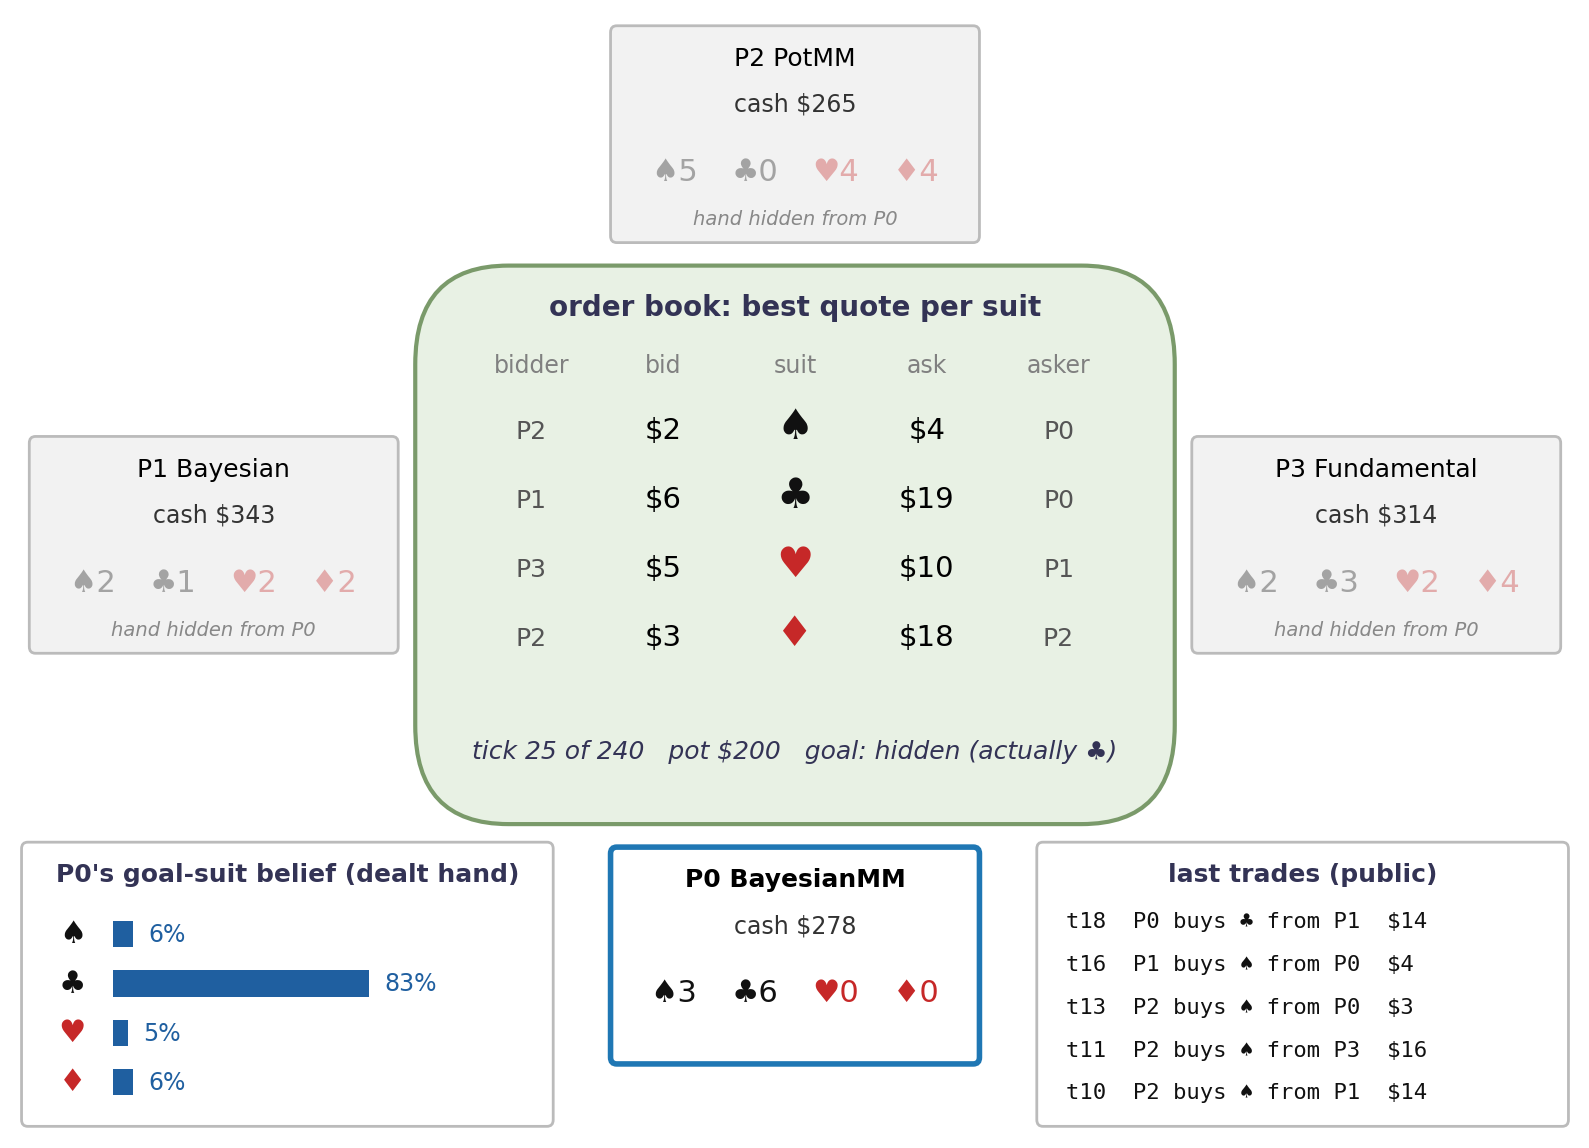
\includegraphics[width=0.6\textwidth]{figgie_snapshot.png}
\end{figure}



\section{Problem and motivation}
In the card game Figgie, you can guess the hidden goal suit by watching who buys what. We measure how much the trades give away, whether reinforcement-learning (RL) agents learn to read them, and whether agents that give away their own hand are easier to beat.

In Figgie, 40 custom cards with no numbers or faces are dealt from one of 12 equally likely decks: one suit has 12 cards,
one has 8 and two have 10. The goal suit is the \textbf{same color \underline{partner}} of the 12-card suit
(\Spade$\leftrightarrow$\Club, \Heart$\leftrightarrow$\Diam), e.g.\ if the deck is
12\,\Spade{} / 10\,\Club{} / 10\,\Heart{} / 8\,\Diam, the goal suit is \Club. Each player pays \$50 into a \$200 pot, and at the end, every \Club{} card pays its holder \$10 from the pot, with the rest (\$100 or \$120) going to whoever holds the most \Club. Players trade continuously by posting prices to buy and sell each suit, and every trade is public. Because goal cards pay out, players pay more for the suit they believe is the goal, so a player who eagerly buys \Club{} is likely to hold many clubs and believe \Club{} is the goal.
Existing approaches, such as \texttt{figment}'s Bayesian market maker, \texttt{Figgie-bot}'s exact inference, and the \texttt{CS224R PPO} agent~\cite{cs224r}, guess the goal suit from their own cards only and ignore what other players' trades reveal.
We ask three questions:
\begin{enumerate}
  \item How much does the public trade history \textbf{reveal} about the goal suit beyond a single hand, and how quickly?
  \item Do agents with memory (minGRU, GRU, transformer) \textbf{learn to infer} the goal suit despite only receiving rewards for profit?
  \item How much does each agent's own action stream reveal or \textbf{leak} about its hand, like a tell in poker, and do the leakiest agents lose the most to a learned best response (exploiter)?
\end{enumerate}

Elo and profit against a fixed field, the only metrics reported for Figgie agents, say nothing about \textbf{why} an agent wins or how robust it is.
Figgie is also a clean testbed for an open question in reinforcement learning under partial observability: does an agent trained only on reward learn to infer hidden state from \emph{other agents' behaviour}? DeepStack and Pluribus~\cite{pluribus} sidestep this by computing beliefs explicitly, while model-free agents with memory are expected to learn them implicitly, but this is rarely checked because in poker or StarCraft the exact belief is intractable. Unlike poker, where hidden information leaks through a few bets in a zero-sum game, Figgie is general-sum (a trade can help both sides) and players reveal information through dozens of priced trades, while the hidden state is tiny (12 possible decks, so the exact belief is easy to compute), isolating the skill of reading other agents. 

\section{Data}
We use no external dataset: all data is simulated in our engine, which implements the standard rules and the CS224R action space~\cite{cs224r} and runs the public agents from two open-source projects~\cite{figment,figgiebot} and the CS224R report, of which the figment and Figgie-bot agents match their original code decision for decision. The simulator logs the true deck and all hands, so each sample carries exact ground truth.

\begin{center}
\begin{tabular}{@{}lr@{}}
\toprule
One game & 240 ticks $\times$ 4 players $=$ 960 decisions \\
Observation / training sample & 69 \texttt{float32} $=$ 276\,B / $\approx$\,300\,B \\
Simulator, measured (1 CPU core) & 11\,ms/game $=$ 85{,}000 decisions/s \\
PPO training, measured & 3{,}800 steps/s $\approx$ 1.1\,MB/s, longest run 33\,M steps $\approx$ 10\,GB \\
Projected, vectorised engine on an RTX~5090 server & $\sim$1\,M steps/s $\approx$ 0.3\,GB/s $\approx$ 1\,TB/h \\
\bottomrule
\end{tabular}
\end{center}

\section{Related work}
Prior Figgie agents (hand-written, Bayesian and evolutionary bots~\cite{figment,figgiebot} and one PPO agent~\cite{cs224r}) are ranked only by profit or Elo, and none is measured for what the order flow reveals or what it leaks.
In market microstructure, Kyle~\cite{kyle} and Glosten--Milgrom model how informed orders reveal private information, assuming rational agents, whereas we measure it for learned agents against exact ground truth.
In multi-agent RL, exploitability has no closed form in multi-player general-sum games~\cite{pluribus}, so learned best responses~\cite{timbers} are the practical substitute, and no estimate exists for any Figgie agent.
In interpretability, probing has shown that AlphaZero encodes human chess concepts~\cite{alphazero_probe}, whereas Figgie gives an exact Bayes-optimal target, so we can investigate whether the network computes the \emph{right} belief.

\section{Preliminary approach}
Baselines are the 1. \emph{hand-only posterior}, the exact best guess from a player's own cards (for belief), and 2. replicated agents.

For question 1, we propose to train a supervised transformer that reads a player's hand plus the public trade history up to tick $t$ and predicts the goal suit. Its gain over the hand-only posterior, $\Delta_{\text{rev}}(t)$, measured in bits of uncertainty about the goal suit (2 bits means no idea, 0 means certain), estimates how much the order flow reveals.

For question 2, we seek to train PPO agents with a minGRU, GRU or transformer over the trade history and open them up with mechanistic interpretability:
(i)~\emph{linear probing}~\cite{probes}, asking whether we can read the agent's belief out of its memory: we decode the true goal suit and opponents' holdings from hidden states at every tick, and score extraction $E_a$ from 0 (it knows only what its cards say) to 1 (it reads the trades as well as our best model),
(ii)~\emph{attribution}, asking which past trades it pays attention to: we find attention heads that track opponents' purchases of a suit, or attribute the GRU's belief to past trades, and
(iii)~\emph{causal interventions}, asking whether changing its belief changes its trading: we steer the hidden state along the ``\Club{} is the goal'' direction~\cite{actadd}, patch activations between matched games~\cite{rome}, and ablate the direction to measure the profit it is worth.

For question 3, leakage $L_a$ is how well a classifier predicts agent $a$'s hand from its actions, in bits over the prior. Exploitability $\hat\varepsilon_a$ is the profit of a PPO best response against three copies of $a$, minus a no-information control.

The central tests are simple: do RL agents learn to read trades ($E_a>0$), does better memory help (no memory $<$ minGRU $<$ GRU $<$ transformer), and do agents that give away more lose more (positive rank correlation between $L_a$ and $\hat\varepsilon_a$)?

By the midterm (3 weeks) we aim to have the revelation bound and first probes of PPO, and by the final report (8 further weeks), the history-aware agents, interventions, leakage and exploitability.

{\footnotesize
\begin{thebibliography}{99}\setlength{\itemsep}{0pt}\setlength{\parskip}{0pt}
\bibitem{figment} mneha05. \newblock figment: a self-play market-making arena for Figgie-style card markets. \newblock \url{https://github.com/mneha05/figment}.
\bibitem{figgiebot} revilo-25. \newblock Figgie-bot. \newblock \url{https://github.com/revilo-25/Figgie-bot}.
\bibitem{cs224r} D.~Li Yang. \newblock Reinforcement learning for Figgie: learning negotiation as a first-class skill. \newblock Stanford CS224R project report, 2026.
\bibitem{kyle} A.~S.~Kyle. \newblock Continuous auctions and insider trading. \newblock \emph{Econometrica}, 53(6), 1985.
\bibitem{pluribus} N.~Brown and T.~Sandholm. \newblock Superhuman AI for multiplayer poker. \newblock \emph{Science}, 365(6456), 2019.
\bibitem{timbers} F.~Timbers et al. \newblock Approximate exploitability: learning a best response. \newblock In \emph{IJCAI}, 2022.
\bibitem{alphazero_probe} T.~McGrath et al. \newblock Acquisition of chess knowledge in AlphaZero. \newblock \emph{PNAS}, 119(47), 2022.
\bibitem{rome} K.~Meng et al. \newblock Locating and editing factual associations in GPT. \newblock In \emph{NeurIPS}, 2022.
\bibitem{probes} G.~Alain and Y.~Bengio. \newblock Understanding intermediate layers using linear classifier probes. \newblock arXiv:1610.01644, 2016.
\bibitem{actadd} A.~M.~Turner et al. \newblock Steering language models with activation engineering. \newblock arXiv:2308.10248, 2023.
\end{thebibliography}
}

\end{document}
